\subsection{Dynamic Graph Operations}
\label{sec:eval:dynamic}

We next compare \project{}'s two representations against three state-of-the-art in-memory dynamic graph systems: Teseo~\cite{teseo2021deLeo}, LiveGraph~\cite{zhu2019livegraph}, and GraphOne~\cite{graphone2019kumar}.
Each of these systems stores the graph entirely in memory and must rebuild it on every restart.
LiveGraph supports mmap-based persistence, but we test it in its default anonymous-mmap mode.
We conduct four experiments: 
(1)~a scalability study that varies writer thread count, 
(2)~an insertion benchmark at each system's optimal thread count across six datasets, 
(3)~a sustained mixed insert-and-delete workload that replays a graph update log, 
(4)~a Graphalytics kernel run after finishing the insertion.

\subsubsection{Insertion Scalability}
We insert edges of graph500-24 (260\,M edges) while varying the number of writer threads from 1 to 72\footnote{We limit the experiment to 1 NUMA node with 96 threads. We did not try scaling past 72 threads to leave room for background compaction threads in systems like Teseo.}.
We define scalability of a system at $p$ threads as the ratio $T(1)/T(p)$, where $T(n)$ is the time taken to insert all edges using n writer threads.
%%%%%%%%%%%%%%%%%%%%%%%%%%%%%%%%%%%%%%%%%%%%%%%%%%%%%%%%%%%%%%%%%%%%%%%%%%%%%%%%
\begin{figure*}[ht]
  \centering
  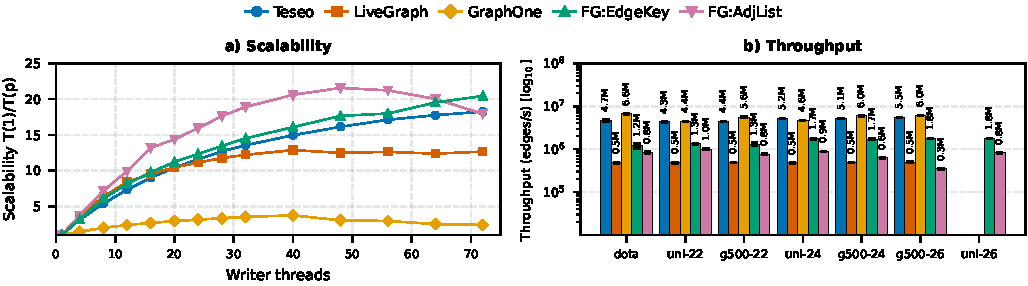
\includegraphics[width=\textwidth]{content/fig/dynamic/dynamic_scalability_throughput.pdf}
  \caption{(a)~Insertion scalability: throughput vs.\ writer thread count on graph500-24.
    (b)~Peak insertion throughput (M~edges/s) at each system's optimal thread count across six datasets.
    Each bar is the mean of 3--5 repetitions; error bars show one standard deviation.}
  \label{fig:dynamic-scaling}
\end{figure*}
%%%%%%%%%%%%%%%%%%%%%%%%%%%%%%%%%%%%%%%%%%%%%%%%%%%%%%%%%%%%%%%%%%%%%%%%%%%%%%%%
\autoref{fig:dynamic-scaling} shows the scalability of each system as the number of writers varies.
GraphOne achieves the highest single-thread throughput (1.69\,M~edges/s) and peaks at 6.3\,M~edges/s with 40~threads, but degrades beyond that point as cross-socket contention on its single write-store ring buffer increases.
Teseo starts lower (0.28\,M~edges/s at one thread) but scales the most consistently, reaching 5.1\,M~edges/s at 72~threads with no sign of
saturation, an 18$\times$ speedup.
LiveGraph plateaus at 32--40~threads near 0.49\,M~edges/s; additional threads yield no further gain.
\project{} EdgeKey reaches 1.7\,M~edges/s at 72~threads, while \project{} Adjacency List peaks near 0.77\,M~edges/s with 48 threads.
Based on these results, we fix GraphOne and LiveGraph at 40~threads and Teseo and both \project{} configurations at 72~threads for all subsequent experiments.

\textbf{Takeaway:} Teseo scales to 72 threads with $\approx 5$ M edges/sec.
\project{} EdgeKey scales to 72 threads, sustaining 1.7\,M~edges/s. Adjacency List peaks at 48 threads, sustaining 0.7\,M edges/s.
Other in-memory systems peak earlier but at higher absolute throughput.

\subsubsection{Peak Insertion Throughput}
Using the optimal thread counts identified above, we measure insertion-only throughput across six datasets ranging from 51\,M to 1.05\,B edges.
\autoref{fig:dynamic-scaling}(b) reports the mean of 3--5 repetitions per configuration.
GraphOne is the fastest system on every dataset (5.6--6.6\,M~edges/s), followed by Teseo (4.3--5.5\,M~edges/s).
Both systems benefit from lightweight append-based write paths: GraphOne appends to a lock-free ring buffer drained by a background archiver, while Teseo uses optimistic latching on fat-tree segments.
\project{} EdgeKey sustains 1.2--1.8\,M~edges/s, roughly 3$\times$ slower than Teseo, reflecting the overhead of WiredTiger's transactional machinery (snapshot isolation and B-tree page splits).
\project{} Adjacency List ranges from 0.35 to 1.0\,M~edges/s; its throughput drops on power-law graphs (graph500-26: 0.35\,M~edges/s), because high-degree vertices produce large adjacency-list values that amplify serialization and page-split costs.
LiveGraph is the slowest at 0.48\,M~edges/s, nearly constant across datasets.

\project{}'s two write layouts present a clear tradeoff. 
The edgekey layout stores one B-tree row per edge; inserts are independent, carry no read-modify-write, and incur essentially zero transaction aborts. 
Its insert throughput scales monotonically to the maximum thread count and saturates near 1.7 M edges/s, bounded by the cost of random-key insertion in a single shared B-tree and the memory \PM{contention?} of one socket.
The adjacency-list layout stores one record per vertex, so every edge insert appends to the source vertex's record. 
The append is a constant-size \code{WT\_MODIFY} delta, but it requires a read of the record's current value.
The write is O(1), but the record is shared; under a power-law degree distribution, concurrent writers issue conflicting modifications to the records of high-degree vertices, and WiredTiger's optimistic concurrency control aborts all but one.
The result is a high rollback rate; each aborted insert retries and re-reads the hot vertex's full overflow-block value, producing >400× read amplification. 
Consequently, adjacency-list throughput peaks at ${\sim}$48 writer threads (${\sim}$0.8\,Meps) and declines beyond that point, because additional writers deepen the contention, capping useful throughput well below the EdgeKey layout.

% Two trends emerge across graph families.
% First, all systems except \project{} Adjacency List achieve higher throughput on larger graphs within the same family (e.g., graph500-24 vs.\ graph500-22), because the fixed overhead of initialization and metadata setup is amortized over more edges.
% Second, power-law graphs (graph500) yield higher throughput than uniform-random graphs of the same scale for GraphOne and Teseo, but the reverse holds for \project{} Adjacency List, whose per-edge cost grows with vertex degree.

\textbf{Takeaway:} GraphOne and Teseo are 3--5$\times$ faster than \project{} EdgeKey on pure insertion, reflecting the cost of WiredTiger's page layout and snapshot isolation.
\project{} Adjacency Lists suffer from high contention under power-law, and do not scale beyond 48 writers in our setup.

%%%%%%%%%%%%%%%%%%%%%%%%%%%%%%%%%%%%%%%%%%%%%%%%%%%%%%%%%%%%%%%%%%%%%%%%%%%%%%%%

\subsubsection{Update Workload}

%%%%%%%%%%%%%%%%%%%%%%%%%%%%%%%%%%%%%%%%%%%%%%%%%%%%%%%%%%%%%%%%%%%%%%%%%%%%%%%%

\begin{figure}[t]
  \centering
  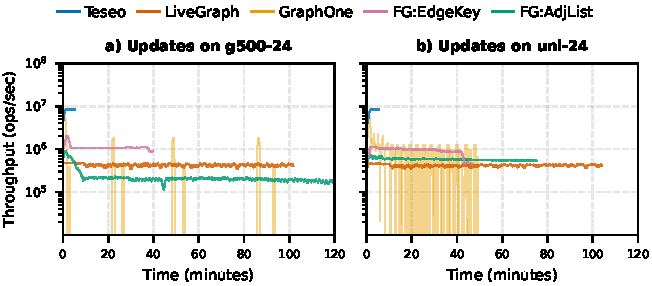
\includegraphics[width=\columnwidth]{content/fig/dynamic/dynamic_throughput_timeseries.pdf}
  \caption{Per-second insertion throughput (60s rolling mean) under updates for a two hour run of a 2.6\,B-operation update log generated on (a)~graph500-24 and (b)~uniform-24.}
  \label{fig:dynamic-timeseries}
\end{figure}
\begin{table}[t]
  \centering
  \footnotesize
  \begin{tabular*}{\columnwidth}{@{\extracolsep{\fill}}lrrrr@{}}
    \toprule
    & \multicolumn{2}{c}{g500-24} & \multicolumn{2}{c}{uni-24} \\
    \cmidrule(lr){2-3} \cmidrule(lr){4-5}
    System & Tput & Mem & Tput & Mem \\
    & (M/s) & (GB) & (M/s) & (GB) \\
    \midrule
    Teseo          & 7.03 & 118 & 6.03 & 119 \\
    FG:EdgeKey     & 1.06 & 483 & 0.91 & 480 \\
    FG:AdjList     & 0.18 & 558 & 0.57 & 457 \\
    LiveGraph      & 0.42 & 726 & 0.41 & 349 \\
    GraphOne       & 0.05 & 162 & 0.87 & 166 \\
    \bottomrule
  \end{tabular*}
  \caption{Update workload: mean throughput \& peak memory.}
  \label{tab:dynamic-update}
\end{table}
%%%%%%%%%%%%%%%%%%%%%%%%%%%%%%%%%%%%%%%%%%%%%%%%%%%%%%%%%%%%%%%%%%%%%%%%%%%%%%%%
The insertion benchmark measures only append throughput.
To evaluate sustained update performance, we generate an update log using the graphlog tool of De~Leo et al\PM{cite the generator}.
Each system replays a precomputed update log (graphlog, aging factor 10) containing 2.60 billion edge operations against the graph500-24 and uniform-24 graphs (final size $\approx$ 260 M edges, 8.9 M vertices). 
The log is $\approx$55\% insertions and $\approx$45\% deletions, with insertions and deletions interleaved so that the graph maintains approximately $|E|$ live edges at steady state.
The first ~10\% of operations form a build-up phase that grows the graph from empty to its full size and is therefore insertion-only; thereafter the workload is a sustained, balanced churn of insertions and deletions that holds the graph at steady-state size.
\autoref{fig:dynamic-timeseries} shows the instantaneous throughput over a two hour run, and \autoref{tab:dynamic-update} reports mean throughput and peak memory for each system on graph500-24 and uniform-24.

Teseo dominates, sustaining 7.0\,M~ops/s on graph500-24 and 6.0\,M~ops/s on
uniform-24, within 30\% of its insertion-only rate.
\project{} EdgeKey sustains 1.06\,M~ops/s on graph500-24, while \project{}
Adjacency List drops to 0.18\,M~ops/s because every deletion must
deserialize, modify, and rewrite the target vertex's full adjacency list.
LiveGraph sustains 0.41--0.42\,M~ops/s, comparable to its insertion-only rate.

GraphOne presents the starkest contrast with the insertion results.
Despite leading the insertion benchmark at 5.95\,M~edges/s on graph500-24,
GraphOne collapses to 0.05\,M~ops/s under the mixed workload, a 115$\times$
drop.
The root cause is deletions: GraphOne's background archiver must locate the
previously inserted edge to set a tombstone, and it has no index for this
lookup.
On power-law graphs, where hub vertices have millions of neighbors, this
search scales with vertex degree and stalls the archiver.
The 134\,M-edge write-store ring buffer fills, and writers block in a
backpressure loop, idle 99\% of the time on graph500-24, with rare
$\approx$16\,M~ops/s bursts.
On uniform-24, where vertex degrees are bounded, GraphOne recovers to
0.87\,M~ops/s.
This behavior matches the findings of De~Leo et al.~\cite{teseo2021deLeo}, who document the same deletion-driven collapse.

\project{} has a larger memory footprint than Teseo and
GraphOne due to WiredTiger's in-memory page structures and MVCC overhead.
LiveGraph uses the most memory on graph500-24 (726\,GB) due to its
copy-on-write versioning of adjacency lists for high-degree vertices.

\textbf{Takeaway}: Insertion-only benchmarks can overstate a system's throughput on real workloads. 
GraphOne, the fastest inserter, collapses by 115$\times$ on power-law graphs when deletions are introduced because its write path lacks an index for edge removal. 
Teseo sustains near-insertion-rate throughput under churn. 
\project{} EdgeKey sustains 1.06\,M~ops/s, and is competitive with LiveGraph.

\subsubsection{Graphalytics performance}
After ingesting a graph, we run breadth-first search
(BFS), PageRank (PR), and weakly-connected components (WCC) kernels directly on the resulting in-memory structure, with each kernel parallelized across all physical threads.
We exclude SSSP, which requires edge weights our generator does not emit, and CDLP (community detection) , which these datasets' property files do not enable.
We run each kernel five times; Table~\ref{tab:analytics-main} reports the \emph{median over the warm runs}, for which run-to-run variation stays below $2\%$. We evaluate the Graph500 (power-law) and \texttt{uniform} graphs at scale factors 22 to 26.

% \textbf{Excluding the cold open.}
% Unlike the purely in-memory baselines, \project{} stores the graph in WiredTiger. 
% Immediately after ingestion, data resides as dirty pages in the buffer cache.
% To ensure that graphalytics kernels run on a stable, consistent, read-only view of the graph, \project{} forces a checkpoint and opens a set of per-thread read-only handles before the first kernel runs.
% The checkpoint makes the first run expensive: it triggers
% \emph{reconciliation}, in which WiredTiger walks every dirty page and reconciles
% its in-memory updates into the page images that constitute the queryable snapshot.
% Since the first Graphalytics kernel invocation triggers the checkpoint, the first run on a freshly built graph includes this one-time cost.
% Because subsequent kernels amortize it, we report steady-state time.

% \project{}'s checkpoint time is, however, far from negligible and grows with graph size: the forced checkpoint takes 59\,s and 68\,s on the SF-22 graphs, roughly five minutes on SF-24 (298\,s / 284\,s), and about 26--27\,min on the billion-edge SF-26 graphs (1536\,s / 1628\,s); opening the read-only handles adds at most 16\,s. 
% The competing systems incur no comparable cost, because they require no reconciliation step: LiveGraph's first run is within noise of its warm runs, and Teseo adds only a few seconds of cache warm-up.
% The cold open is therefore the price FlexoGraph pays \emph{once} to convert a write-optimized store into a consistent read snapshot that subsequently serves analytics at in-memory speed.

\textbf{Results.}
On steady-state kernel time, FlexoGraph (AdjList) is the only system that is fast and stable across all three kernels and all scales, never degrading dramatically as graph size increases.
Teseo runs BFS the fastest (0.04--0.6\,s), with FlexoGraph close behind (0.14--1.4\,s), but Teseo's PageRank and WCC degrade sharply with size (up to 50\,s for PageRank and 16\,s for WCC on \texttt{uniform-26}), whereas FlexoGraph's
PageRank stays at 5.7 and 10\,s on the SF-26 graphs, $3$--$5\times$ faster than
every other system. 
LiveGraph is competitive on \texttt{uniform} WCC (as low as 0.06\,s), but scales poorly on power-law inputs (BFS 7.5\,s, WCC 10.5\,s on \texttt{graph500-26}). 
GraphOne is the slowest reader throughout, and its WCC is catastrophic (346 and 401\,s on the SF-26 graphs), confirming that its read path does not recover the ground lost on updates.
Finally, we include the \texttt{split\_ekey} layout to quantify the layout choice: optimized for ingestion, it is up to three orders of magnitude slower for analytics (BFS 640\,s vs.\ 0.37\,s for adj on \texttt{graph500-24}), which is precisely what motivates the read-optimized adj layout used everywhere else.

\textbf{Takeaway.}
\project{} (AdjList) is the only system that delivers fast, stable analytics across all three kernels and all scales.
Teseo runs BFS faster but its PageRank and WCC degrade sharply at scale; LiveGraph is competitive on uniform WCC but scales poorly on power-law inputs; GraphOne's read path is the slowest throughout.
The EdgeKey layout, optimized for ingestion, is up to three orders of magnitude slower on analytics, confirming that layout choice is the dominant factor.
This steady-state performance comes at a cost: \project{} pays a one-time checkpoint to reconcile dirty pages into a read snapshot (up to 27\,min on billion-edge graphs), a penalty the in-memory systems avoid entirely.